\documentclass[tikz,border=10pt]{standalone}
\usepackage{tikz}
\usetikzlibrary{shapes.geometric,angles,quotes,calc, intersections} % Add this for angle labels

\begin{document}
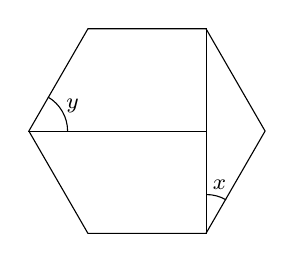
\begin{tikzpicture}[scale = 1]
    % Draw the hexagon
    \node[regular polygon, regular polygon sides=6, minimum size=3cm, draw] (p1) {};

    %labeled vertices of hexagon
    \coordinate (A) at (p1.corner 1);
    \coordinate (D) at (p1.corner 2);
    \coordinate (K) at (p1.corner 3);
    \coordinate (B) at (p1.corner 5);
    \coordinate (C) at (p1.corner 6);
    
     % Draw vertical line
    \draw (A) -- (B);

    %horizontal line
    \path[name path=horizontal] (p1.corner 3) -- (p1.corner 6);

    \path[name path=line1] (p1.corner 5) -- (p1.corner 1);
   
    \draw[name intersections={of=line1 and horizontal,by={Int1}}] (p1.corner 3) -- (Int1);
    
    \pic [draw, "\footnotesize $x$", angle eccentricity=1.3, angle radius=0.5cm] {angle = C--B--A};
    \pic [draw, "\footnotesize $y$", angle eccentricity=1.3, angle radius=0.5cm] {angle = Int1--K--D};
    
\end{tikzpicture}
\end{document}